
\labtitle{Fall 2015}{1}{Monday, August 31/Tuesday, September 1}

\section*{Introduction}
\subsection*{Agenda}
\begin{itemize}
    \item Self/Student Introductions!
    \item Brief discussion of course and breadth of its material.
        \begin{itemize}
            \item Algorithms
            \item Data Structures
            \item Runtime Complexity
        \end{itemize}
    \item Where will this course take you?
        \begin{itemize}
            \item Interview preparation, jobs
            \item Smart, informed coding choices and profiling
            \item Start to doubt the world around you. Beware of black box code!
            \item Theory-land
        \end{itemize}
    \item Course caveats (at least in past semesters):
        \begin{itemize}
            \item Lots of math, for Big Oh proofs/statistical analysis later on.
            \item Java, JUnit (If you don't feel comfortable, please let me know! I will try to help.)
            \item Less hand-holding.
            \item Walk the walk! If you don't do the work, you're going to have a hard time.
        \end{itemize}
\end{itemize}
\begin{figure}[h]
    \centering
    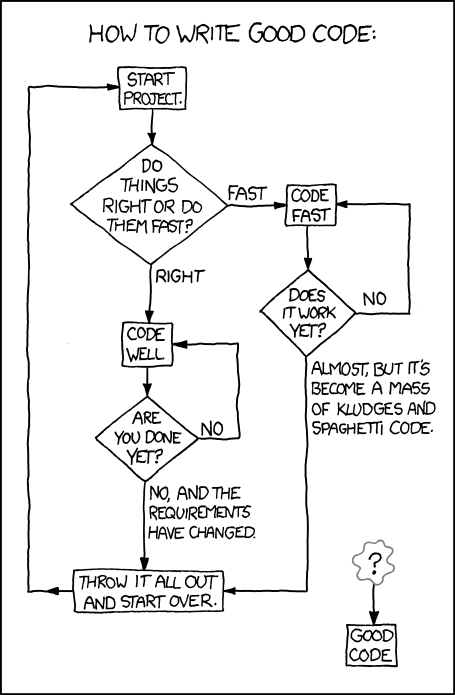
\includegraphics[width=\textwidth*5/16]{good_code}
    \caption*{\underline{\textit{\href{http://xkcd.com/844}{XKCD: 844}}}}
\end{figure}

\newpage

\subsection*{Problem 1} 

\textbf{Unique Character Strings:} Given a string of length $n$, determine whether it contains all unique characters - or, whether any characters are used more than once.\\

\textit{Tips:} Guess the lower-bound! What is the limit on the fastest runtime algorithm that anyone can formulate for this problem?\\

\textbf{Naive Solution.} Iterate through each character $c$ in the string $s$. For each such $c$, iterate starting from the next character to the end of the string. If a duplicate character appears, return false. Otherwise, return true.\\

\begin{minted}[ linenos,
                framesep=5mm,
                fontsize=\footnotesize,
                bgcolor=bg]{java}
    //naive solution
    boolean hasNoRepeats(String s) {
        for (int i = 0; i < s.length(); i++) {
            for (int j = i+1; j < s.length(); j++) {
                if (s.charAt(i) == s.charAt(j)) {
                    return false;
                }
            }
        }
        return true;
    }
\end{minted}
\mbox{}\\

\textit{Runtime:} Quadratic.\\

How might you guess that you could improve this runtime? Notice how this algorithm will repeat itself by examining the same parts of the string over and over again. Trying to avoid pointless repetition is a key to success.\\

\textbf{Alternate solution.} Suppose the string $s$ only contains characters from the English alphabet. Create a boolean array $B$ of size $26$, with all values initially false. Iterate through $s$ and examine each character in order. Suppose that at any particular point in the iteration WLOG you have the $i$th character in the alphabet. Check if $B[i]$ is true. If it is, return false. Otherwise, set it to true and continue. At the end of the iteration, return true.\\

\textit{Runtime:} Linear (in terms $n$). Space usage is constant.\\

\textit{Suggested improvements:} Use a bitstring of maximal size $\log m$ instead of an array. ($m$ is size of the alphabet.) Example solution in C shown on the next page, \textbf{for the 240 folk.} (It's ok if you don't understand. C is not covered in this course!)\\

\textbf{Alternate solution 2.} Iterate through each character of the string and add each to a set $S$. If $S$ already contains the character, return false. Otherwise, return true.\\

\textit{Runtime:} It depends! How is the set implemented? Is it a black box? If you don't know the runtime of set add/contains, you can't use this result.\\

\begin{minted}[ linenos,
                framesep=5mm,
                fontsize=\footnotesize,
                bgcolor=bg]{c}
    // pr0.c
    // Implementation of alternate solution 1.
    // READ IF CURIOUS. NOT COVERED IN COURSE MATERIAL.
    // Returns 1 if string has no repeat characters.
    // Otherwise, returns 0 if it finds any.
    // 
    // @param s - string of lowercase alphabetical chars

    int hasNoRepeats(char *s) {
        unsigned int b = 0;

        for (int i = 0; i < strlen(s); i++) {
            int offset = s[i] - 'a';

            if (1 & b >> offset) {  //Examine the ith bit.
                return 0;           //If set, duplicate found!
            }

            b |= (1 << offset);     //Mark bit as found.
        }

        return 1;
    }
\end{minted}
\mbox{}\vspace{20pt}


\subsection*{Problem 2}

\textbf{Anagram Strings:} Given two strings, determine whether they are anagrams of each other.

\begin{center}
    \texttt{TOMMARVOLORIDDLE} $\longleftrightarrow$ \texttt{IAMLORDVOLDEMORT}\\

    \textit{The above are anagrams of each other!\\ (Sorry if I spoiled book 2 of Harry Potter for you...)}
\end{center}

\textbf{Solution 1.} Suppose the two strings are $s_1$ and $s_2$ and we are allowed to modify them. Compare their lengths. If unequal, return false. Compare the strings. If they are equal, return true. Iterate through $s_1$. For each character $c$, try removing $c$ from $s_2$. If $c \notin s_2$, return false. When finished, if $s_2$ is not empty, return false. Return true otherwise.\\

\textit{Runtime: } Quadratic. At each iteration we search in $s_2$, doing $n + (n-1) + (n-2) + ... + 1 = \frac{n\cdot(n+1)}{2}$ total work in the worst case.\\

\textbf{Solution 2.} Sort both strings and compare them for equality.\\

\textit{Runtime: } It depends. There are variety of sorting algorithms out there, from the speedy quicksort to the \textit{infamous} bogosort! Using quicksort or any comparison based sort, the lower bound will be linear-logarithmic ($n \log n$). You'll learn more about this later in the course.\\

\textbf{Solution 3.} Suppose the two strings are $s_1$ and $s_2$ and that both have a fixed alphabet (English). Create two arrays, $A$ and $B$ and initialize their entries to $0$. Iterate through $s_1$. For each character $c$, if it is the $i$th letter in the alphabet, increment $A[i]$. Repeat for $s_2$, using $B$ instead. When finished, iterate through $A$ and $B$ at the same time,
comparing the values of the entries. If for any $i$, $A[i] \neq B[i]$, return false. Otherwise, return true when finished.\\

\textit{Runtime:} Linear, and constant space. Observe that the first loop runs $n$ times. The second loop runs a constant number of times, also doing a constant amount of work.\\

\textit{Suggested improvements:} To improve space usage, instead of having two arrays - create one. Each time a character shows up in $s_1$, increment by 1. Each time a character appears in $s_2$, decrement by 1. In the second loop, check for nonzero entries.\\

\begin{minted}[ linenos,framesep=5mm,fontsize=\footnotesize,bgcolor=bg,mathescape]{java}
    
    /**
     * Returns whether two strings are anagrams of each other.
     *
     * @param s1, s2 - the input strings. Assumed to contain
     *                 only letters of the English alphabet.
     */
    boolean areAnagrams(String s1, String s2) {
        if (s1.length() != s2.length()) {
            return false;
        }
        if (s1.equals(s2)) {
            return true;
        }

        int A[] = new int[26], B[] = new int[26];
        for (int i = 0; i < s1.length(); i++) { //Compute the histograms of $s_1$, $s_2$.
            A[s1.charAt(i) - 'a']++;
            B[s2.charAt(i) - 'a']++;
        }

        for (int i = 0; i < 26; i++) {          //Compare histograms.
            if (A[i] != B[i]) {
                return false;
            }
        }

        return true;
    }

\end{minted}
\mbox{}\vspace{20pt}
\subsection*{Problem 3}

\textbf{Dutch National Flag: } Given $n$ balls of three colors - say red, white, and blue - arranged randomly in a line, sort them as quickly as possible into contiguous groups of red, white, and blue, with the groups in that order.\\

\begin{figure}[h]
    \centering
    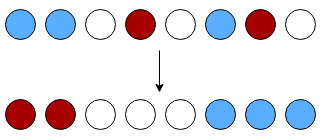
\includegraphics[width=\textwidth*3/8]{dutch_flag}
\end{figure}

\textit{How fast can generic sorts do this?}\\

Selection and insertion sort can do this in quadratic time. Not exactly the best choice.\\

Mergesort can solve this in linear-logarithmic time... but not in-place.\\

Quicksort can do the sort in average-case linear-logarithmic time and worst-case quadratic time, in-place.\\

\textbf{Linear-time algorithm.} Suppose the array $A$ is given as an input, which contains the initial ordering of the balls. Assume that red balls are represented as $0$'s, white $1$'s, and blue $2$'s. Create an array $B$ of size $3$, where the entries are initialized to $0$. Iterate through $A$. For each occurrence of a colored ball, increment the corresponding entry in $B$. When finished, iterate through $B$. For $i=0$, output $B[0]$ red balls - and so forth.\\

\begin{minted}[ linenos,framesep=5mm,fontsize=\footnotesize,bgcolor=bg,mathescape]{java}

    //
    int[] dutchNationalFlagSort(int[] A) {
        int B[] = new int[3];

        for (int b : A) {
            B[b]++;
        }

        int count = 0;
        for (int i = 0; i < B.length; i++) {
            for (int j = 0; j < B[i]; j++) {
                A[count++] = i;
            }
        }

        return A;
    }
\end{minted}
\mbox{}\vspace{20pt}

The above is an implementation of \textbf{counting-sort}, which you'll learn later on (probably in 320.)
